\chapter{Discussion}
The following chapter consists of an evaluation when combining the obtained results, followed by a discussion of the generalizability of the datasets, the correctness of the implementation, and future work.
\section{Evaluation of Results}
\subsection{Execution Time Analysis}
As evident by FPDE's performance, compressed data should not be seen as merely disorganized, as there are several opportunities to create structure and optimizations for various purposes. 

The results indicate several advantages of using FPDE in terms of execution time, and, on average, all investigated operations perform better using FPDE compared to the baseline. However, the operation's execution time is highly dependent on contexts such as geometry sizes, intersection type, add vertex index placement, among others. Since FPDE outperforms the baseline in all of these cases, it implies that if the aim is minimal execution time, even though the variability in performance is extensive, it is more beneficial to utilize a scheme like FPDE over conventional compression schemes. 


Nevertheless, increased operability comes at the expense of compressibility. As shown in the results, the size proportions between the induced overhead and the original shape data vary significantly between the datasets, from around 25\% to 63\%, decreasing with the average vertex count of the datasets. Likewise, the relative execution time gains for the operations are higher for complex geometries. However, while simple geometries only experience a speedup of approximately 19\% for intersection when the geometries' bounding boxes overlap, they still achieve an average speedup by a factor of 35.7 when extracting the bounding box. Considering these variations, the balance of the time-space trade-off relies on the geometry size and the type of operation. While the additional overhead for simple geometries might not be worth the tiny gain in execution time for intersection, it may be worth it when getting the bounding box. Alternatively, it can be practicable to toggle the operability support on a per-operation and per-shape basis, allowing the algorithm to utilize partial decompression for situations where the performance gains are most significant and, otherwise, prioritize size and avoid the metadata overhead. It is also worth noting that the overhead induced in the thesis can probably be well reduced in future work, such as by using a quadtree as proposed in Section \ref{sec:quadtreechunk}.


However, some operations do not interfere with time and space trade-offs. \textit{Add Vertex} achieves a similar execution time gain as the bounding box operation, without any additional metadata needed. In this case, the operation is considered a two-way benefit and can thus be used without any trade-off considerations. As a side note, in practice, the partial "re"-compression when adding a vertex is likely very beneficial in GIS editing tools since modifying individual vertices in shapes is a frequent operation.








% i.e., that intersection utilizes the natural forming of chunks in order to perform initial low-resolution filtering using the chunks' bounding-boxes. However, since there is an evident time-space trade-off, adding more operations will lead to a lower compression ratio since more space must be allocated for metadata and other optimizations.



% DONE Overall, as the results show, all operations investigated benefits from partial decompression

% (DONE) It is apparent that compression should not be treated as a black box, since the underlying structure of the algorithms may allow for optimizing of the operations. As evident by FPDE when intersection utilizes the natural forming of chunks in order to perform initial low-resolution filtering using the chunks' bounding-boxes.

% (DONE) There exist several possible optimizations which can be applied to the algorithm used for returning the intersecting shape. For instance, the odd-

% (DONE) Performance of operation and compression depends on the context of geometries 

% (DONE) Decompress and Compress slower than baseline. Operations MUCH faster on average random geoms.

% (DONE) Entropy, adds additional overhead in its conversion 

% (DONE) Fined grained with limit, however performance is changed by this as per graph.

% Different methods of creating chunks, ex. split by quadtree, minimize the overlap between chunks

% Chunks are formed automatically pretty good, but infer maxiumum number of chunks for homogeneous chunks. 

% For Add Vertex the partial "re"-compression is likely greatly benefitically in GIS editing tools, since modifying individual vertices in shapes is likely a common operation.


\subsection{Compressibility Analysis}
\label{sec:compressanalys}
As concluded in the results section, maps data has the potential to be compressed beyond the limits of general-purpose compression algorithms, such as \textit{gzip} and \textit{bzip2}, by exploiting the domain. This section reasons about why the implemented compression scheme performs well and proposes additional ideas, in accordance with the conclusions obtained through the thesis, which may improve the compression further.

Firstly, using arbitrary precision floating-points is probably not needed since a precision higher than a certain decimal digit is likely noise due to the limited accuracy of the data collection methods. By instead quantizing the coordinates to integers, higher compression ratios can be achieved. However, if 64-bit double precision is required, the results indicate that compression by delta encoding the integer representation may still be worthwhile.

\begin{figure}[H]%
    \centering
    \subfloat[\centering Chosen delta bit size per geometry.]{{\includegraphics[width=6.9cm]{images/sweden_100000_optimal_delta_size.png} }}%
    \qquad
    \subfloat[\centering Required bit size per delta.]{{\includegraphics[width=6.9cm]{images/sweden_100000_per_deltas.png} }}%
    \caption{Bit sizes for the deltas and chosen delta bit size in 100 000 random geometries from the \textit{Sweden All} dataset.}%
    \label{fig:swedenbitsize}%
\end{figure}

The delta encoding likely performs well since geometries usually only span a small area of the world, while the integer decomposed coordinates can store distances across the globe.

For map data with seven decimal digits of precision, an accuracy of 1.11 cm is stored, and with each digit removed, it is scaled by a factor of ten. Because maps data is based on several collection methods, with varying precision, it is unlikely that most of the data uses centimeter-level precision and is thus noise in the data. Noise is unsuitable for compression, as it is uniformly distributed and thus no statistical redundancy can be utilized. If those cases can be stripped of the least significant bits containing the noise, entropy coding can be enhanced. One proposition is to infer the precision of the sampling from the data collection method to determine the needed decimal accuracy. Depending on the maps data provider, it might be of interest to perform lossy compression dependent on the geometry size. As seen in Figure \ref{fig:swedenbitsize}, the average delta bit-length for \emph{Sweden All} is 13.2 bits, corresponding to approximately half a meter in real-world measurements. For \emph{Admin Borders}, with a delta bit-length of 20.2 bits or approximately 800 m,  it is unlikely that centimeter-level precision is required, and thus some of the least significant bits can be removed.

With a size of 13.2 bits, a total of 9400 deltas, and the highest precision of $\pm 0.0004700$, longitude/latitude degrees can be represented. Thus, a reduction to 4705 deltas is required to scale down one bit, corresponding to halving the distance in real-world measurements. Here, predictor functions can be used to estimate the deltas and then code the residuals. Since some map structures are very similar, such as buildings and roundabouts, storing the structure as a global model and assigning each shape to a specific model by a constant in the header could likely reduce the size further. 

An interesting observation is that chunks are formed when a delta is large compared to its geometry context, which means that the distances between the chunks are larger than the deltas. This can also affect the execution time, since the chunk bounding boxes get inflated when they span to the next linked chunk. Instead, the linking segments between chunks could be placed in their own bounding boxes.

%An interesting case to examine is when the floating-point exponent bits differ by one when using default FPD encoding, potentially resulting in a significantly larger delta.  To avoid this, the exponent and mantissa could be delta encoded separately.

It may be interesting to investigate whether shapes having an uneven distribution of deltas may result in less compression, such as shapes clustered in certain regions but otherwise sparse. One solution may be to have a variable delta bit-length, where each chunk header contains an extra bit specifying whether a new delta bit-length follows.

Additionally, it is possible to describe the deltas in polar coordinates, where the error of the angle scales with the radius. In this case, the radius is delta encoded as is, while the angle is delta encoded followed by a truncation of decimals, depending on the tolerated error margin. This makes implementing approximation of large distances trivial.







\subsection{Relevance in the Real World}
The thesis has demonstrated that it is possible to reduce the size of maps data from the commonly used WKB to a compressed format by applying quantization, delta encoding, and entropy encoding. If sacrificing compression ratio and embedding metadata, operability support can be added to improve the querying speed of common operations. 

If it is worth sacrificing storage for operability is difficult to decide without more knowledge about the pipeline architecture. If billions of intersection queries are running and I/O is not the bottleneck, then total time can be saved.

However, I/O is commonly the bottleneck in systems, and therefore compressing data to the fullest in order to minimize the I/O use may be preferred \cite{fpzip}. Although, it is worth noting that the overhead induced in the thesis can likely be well reduced and, by adding a toggle-bit for operability integration on a per-shape basis, only one bit is added in comparison to full compression when integrated operability is disabled.


\section{Dataset Properties}
% Why do we see different results?
%more accurate shapes more vertices
For the integration of operations to be beneficial, the benefits should apply to a significant portion of the data. The results show that the improvements increase rapidly with the vertex count, a result of having a higher number of chunks, but simple shapes also benefit from partial compression. However, for simpler shapes, the size of the induced overhead for operability impacts the compression ratio to a greater extent. 

\begin{figure}[H]
    \centering
    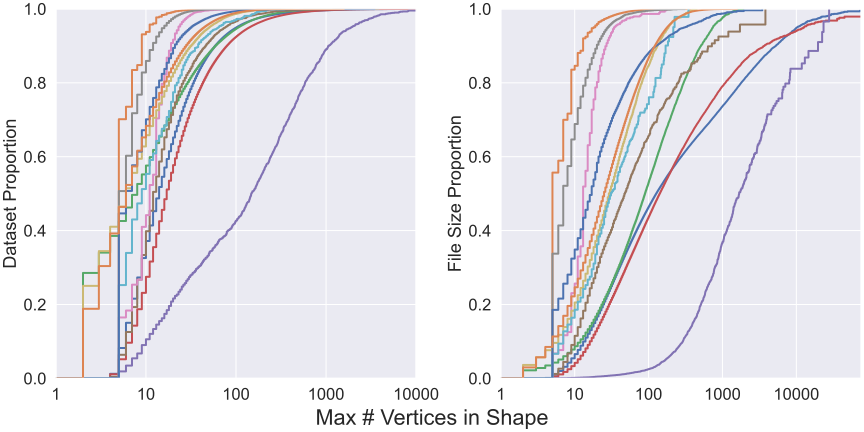
\includegraphics[width=15.15cm]{images/data_distrb_sweden.png}
    \caption{Cumulative distribution of the vertex count for the geometries in \emph{Sweden All}, separated by OSM-tags. The right plot is weighted by the number of vertices, indicating how the overall size is distributed.}
    \label{img:data_distrb_sweden}
\end{figure}

The average vertex count for the geometries in \textit{Sweden All} is 16.4 and 75\% of all shapes have less than ten vertices. Therefore, the percentage of shapes where the gain in execution time significantly outweighs the size overhead is rather low. 

As seen in Figure \ref{img:data_distrb_sweden}, illustrating the distribution of the vertex count for shapes of different types within the dataset, the type of the shape correlates with the average number of vertices. It is logical that geometries covering a large area of the world are constructed using more vertices to increase the detail. Additionally, there are many more houses than country borders, which means that the average is more influenced by simple geometries. Also, complex structures are commonly split into multiple simpler geometries.

The distribution likely also depends on how the spatial data is structured, and our sampling of OSM data might not be a good representation of how other maps services structure their data. For instance, other providers' datasets may consist of many complex geometries due to a higher resolution. It may also be that even though there are fewer geometries in which integrated operability is motivated, the gains are still important. Therefore, it is crucial to obtain precise querying data to identify the exact bottlenecks.

\subsection{Intersection Queries}
% Svårt att hitta faktiskta intersection queries, vi bara approximerar
Due to the high variance in the intersection results, one possible error source is the real-world representativity of the intersection data used in the evaluation. As described in Section \ref{sec:intersectiondataintro}, there are a number of different cases of intersection. The execution time may vary depending on both the intersection case, characteristics of the shapes, and the intersecting region.

Extracting queries representative of real-case use by maps service providers is not trivial. Since intersection queries are commonly used when validating the map, the nature of the queries depends on the validation process and the internal structure of the maps data. A log of recent queries along with the involved geometries would be ideal, but due to secrecy, such data is not publicly available.

It may not be as accurate to construct the intersection queries by picking one geometry at random and finding its neighboring shapes, as done in the thesis, but the queries may still be used as an approximation of real-use scenarios. For example, finding all intersecting geometries and their type is likely frequently used to ensure that no constraints are violated, such as a road intersecting with an ocean.

Additionally, intersection queries tend to involve one complex and one simple geometry for the context \(Contained\). For example, when calculating whether a geometry is within a larger area, such as a state, province, or country, represented by their administrative boundaries. Such queries will benefit significantly from integrated intersection capabilities. This is supported by Table \ref{tab:context_distribution}, showing that the \textit{Contained} case is most common when a complex and a simple geometry is involved.

\begin{table}[H]
\centering
\begin{tabular}{lccc}
\hline
Size & Contained (\%) & Disjoint (\%) & Crossing (\%) \\
\hline
L/L & 0.23 & 2.0 & 11 \\
M/L & 0.13 & 1.5 & 3.1 \\
M/M & 0.08 & 0.66 & 1.4 \\
S/L & 9.9 & 6.9 & 5.2 \\
S/M & 2.9 & 4.5 & 3.7 \\
S/S & 7.6 & 30 & 10 \\
\hline
\end{tabular}

\caption{Context and geometry complexity distribution for the intersection query pairs used in the evaluation.}
\label{tab:context_distribution}
\end{table}

Table \ref{tab:context_distribution} also shows that the distribution of various intersection query types is not uniform, and some accounts for less than 0.1\%. In these situations, it is essential to collect enough data so that even a tiny percentage is a sufficient representation of generality.


The same table shows that some of the intersection query types occur more frequently than others. If a specific query rarely occurs, the results might not have enough support to draw general conclusions. For example, some types of intersection queries are very infrequent for the M/M category, such as \textit{Contained}, which only accounts for $0.08\%$ of the queries.
% \todo{hur många är totalt här? eller skriv hur mycket en procent motsvarar?}



\section{Validity and Correctness}
\subsection{Representativity of Baseline}
Since the implementation is written in Python, which is a mixture of wrappers that execute C code and interpreted Python code, comparing performance and generalizing the results to compile-based languages, including optimizing/JIT compilers, is tricky. When developing the baseline and the extended solution, special care has been taken to ensure that the implementations are as similar as possible in the common parts. Therefore, the results obtained are likely to translate well to speed-optimized languages, but an implementation of FPDE in such a language is required to further verify the results.

Due to the uncertainty regarding performance induced by the language, an alternative language-independent metric of interest is the fraction of unfolded chunks. As discussed in Section \ref{sec:intersection_results}, for the intersection queries used in the thesis, the integrated intersection operation only decompresses around 20\% of the complex geometries. The only way for a baseline implementation to be faster is if the execution time needed for filtering and finding the relevant chunks is larger than the decompression time of the remaining 80\% of chunks. This is unlikely since the operations performed for finding the chunks are rather lightweight. Additionally, irrelevant data can be discarded at an earlier stage, and therefore the intersection algorithm is only performed on a subset of the data. Smaller input is expected to decrease the execution time. Also, when delta encoding is combined with entropy encoding and predictor functions, or other compression techniques, an increase in decompression time is inevitable, and the benefits of partial decompression increase with the decompression time.

\subsection{Implementation Correctness}
Even though FPDE provides a robust solution to a compression format and the specified operations, some cases can lead to unexpected behavior. 

 The intersection algorithm specified in Section \ref{sect:chkintersect} can return the incorrect result if certain types of multipolygons are involved. Suppose a multipolygon, consisting of polygons \(X_1\) and  \(X_2\), intersects with a polygon \(Y\) by \(X_1\) being fully contained in \(Y\), and \(X_2\) being entirely outside it. Additionally, the bounding box of the multipolygon is contained within the bounding box of \(Y\). The correctness of the result in this scenario depends on whether the random point for the ray-sending strategy, outlined in Section \ref{sec:fully_contained}, comes from \(X_1\) or \(X_2\). If sent from the outer one, the ray crosses an even number of edges, and the returning intersection shape will be empty. On the other hand, if the ray is sent from the inner one, the ray will cross an odd number of edges, and it will correctly return \(X_1\). The solution to this inconsistency is to treat \(X_1\) and \(X_2\) as individual entities in the algorithm and return the combined result of each. 
 
 Another case where the intersection algorithm can return incorrect results is with polygons containing inner holes. Suppose a setting where two polygons \(X\) and \(Y\) intersect. \(X\) contains an inner hole \(X_i\), which does not intersect with any of the edges of \(Y\) but is fully contained within the overlapping area of \(X\) and \(Y\). Since the algorithm only constructs the returning shape by traversing the intersection points, the area of the inner hole will incorrectly be excluded from the returning shape. This is solved by decompressing one point in all inner holes with a bounding box overlapping with the returned shape's bounding box and then adding the holes fully inside the returning shape using the ray-sending strategy. 
 
 
 In addition, the algorithm does not support self-intersecting polygons, but as mentioned in Section \ref{sec:intersection}, such geometries are commonly considered errors in spatial data. It is also worth mentioning that the intersection algorithm passes over 99.9\% of all intersection queries from the various datasets in Section \ref{sec:intersection_results}, confirming that these cases of intersection are very rare.


  Furthermore, the formats for representing floating-point coordinates, described in Section \ref{sec:delta_mod}, can result in inaccurate delta values if calculated on coordinates with a longitude degree difference greater than 180. In this case, the floating-point representations cannot fit the delta value, and it will lead to overflow. However, this occurrence is rare in spatial data since it would mean that geometries span half the globe or segments cross the \textit{International Date Line}. For the \textit{variable precision float} format, it can be corrected by extending the exponent section by one bit, and for the \textit{32-bit integer decomposed coordinate} format, by using modular arithmetic on immediate calculations.


\section{Extending Supported Operations}
% How can what we learned be used to further improve other operations?
The operations implemented in the thesis are few compared to the many operations commonly present in geometry libraries. For the format to be adequate for real-case use, it must be possible to implement all operations.


All operations should be able to be implemented following the baseline approach, where the entire geometry is first decompressed, followed by utilizing an existing library function. Accordingly, extending a compression format with more operations can be done iteratively. The ones that bottleneck the system, or are less challenging to implement, could be optimized first, while the non-optimized ones utilize the baseline strategy.

Furthermore, the three implemented operations; \textit{bounding box}, \textit{add vertex}, and \textit{intersection} are characterized by being \textit{constant}, \textit{modifying},
and \textit{binary} operations. Thus, many of the principal components in the implemented operations can be reused to extend the supported operations.
For example, the idea of utilizing the chunks' bounding boxes for intersection can be used to add integrated support for \textit{union}.  Most non-modifying unary operations can be pre-calculated and stored as metadata, and many modifying unary operations can be performed on a per-chunk basis.

\section{Answering the Problem Formulation}
Based on the results and implementation process, the research questions of the thesis can be answered.

\begin{description}
    \item[Q1:] Is it possible to perform operations on compressed geometric data without decompressing the entire geometries?
\end{description}

\noindent Yes, performing operations by partially decompressing geometric data is possible, as evident by the intersection queries only decompressing a fraction of all chunks, and adding a vertex only altering the relevant data sections.
The value of implementing partial decompression depends heavily on the distribution of complex geometries (shapes consisting of many vertices) within the datasets and the performance of the used compression algorithm. The effects are more evident for slower compression algorithms, such as when combining delta and entropy encoding, since the integrated format only unfolds a fraction of the compressed coordinates. 

Additionally, extra overhead is introduced both in terms of extended metadata and the computations needed to determine which data sections to decompress. The number of vertices affects the number of chunks, and with a larger number of chunks, the gains are usually higher since a greater portion of the geometry avoids decompression.

\begin{description}
    \item[Q2:] How can domain-specific constraints and structures, in the context of maps, be exploited to improve the performance of operations and geometry compression?
\end{description}

\noindent Several domain-specific properties can be used to improve the operability and compression performance of maps data, such as representing coordinates as 32-bit integers, delta encoding coordinates, dividing the shapes into mostly non-overlapping chunks, and assuming no self-intersection.

Noise in the data can be reduced by quantizing the coordinates to seven decimals (one centimeter precision) and concatenating the integer and decimal part into a 32-bit integer, resulting in a more compact storage form and higher compression. Delta encoding of map coordinates also performs well, due to individual geometries usually only spanning a fraction of the world. Additionally, simply dividing the shapes into chunks containing a subsequence of all vertices, i.e., a continuous slice of the index vector, results in a division that can be used to improve the performance of operations. Furthermore, by assuming that there are no self-intersecting geometries, any found intersection must be between two separate shapes, reducing the complexity of implementing the intersection operations.  

\newpage
\section{Future Work}
The following section contains explanations of several ideas that can be explored to extend the thesis in future research. Additionally, Section \ref{sec:compressanalys} also presents concepts and motivations for improving the compression ratio further.
\subsection{Implementation in High-Performance Language}
Because the thesis implementation is written in Python, it is not applicable for practical use in a high-performance context. As described earlier, the baseline is also implemented in Python, and thus the results indicate a relative gain and that there exist cases where only a fraction of all chunks need to be decompressed. In order to compete with state-of-the-art geometry compression and further evaluate the potential applications on a large scale, the concepts in the thesis need to be implemented in a high-performance language. Since much of the current implementation is just logic-based and bit-operations, i.e., most of the code for the compression format does not utilize Python libraries, the translation should be straightforward.

\subsection{Further Reducing Interobject Redundancies}
%Kollar bara på enskilda geometrier: sämre kompression
%Spatial parquet column based, kollar på mängd geometrier
It is clear from the results that, in terms of entropy encoding, the deltas are close to the limit calculated using Shannon's source coding theorem when using Huffman encoding. Arithmetic encoding may be able to reduce the size further, by compressing whole chunks rather than individual deltas.  However, the potential additional size reduction is not expected to be groundbreaking.

Therefore, in order to further compress the deltas, which for complex geometries account for the majority of the data, alternative techniques are required. One proposition, when working with maps data, is to differentiate between geometry types. For example, buildings consisting of four vertices are very common, and for such buildings, the deltas should be similar. It would be of interest to examine whether using different probability tables for each geometry type (road/building/water) would result in a distribution that is more skewed and beneficial for entropy encoding. Furthermore, predictor functions based on the geometry type should, for geometries with a standardized structure, be able to reduce the size further.

\subsection{Parallelization of Algorithm}
% Clusters, optimize by partial computation
With the increase of parallel and distributed computing, altering algorithms to enable compatibility with big data environments allows for both horizontal and vertical scaling \cite{parallell}. Vertical scaling utilizes multiple cores or GPUs to divide the workload locally, while horizontal scaling distributes the workload to a number of computers.

In both cases, the workload is divided between workers, and thus it must be possible to decompose the work into non-overlapping parallel tasks. Since FPDE consists of independent chunks, it should be possible to parallelize both the compression, decompression, and some of the operations. For instance, the intersection operation can be divided by assigning each worker to a section of the common bounding box and merging the partial computations.


\subsection{Extended Investigation of Chunking}
While conducting the various performance assessments, it was discovered that the performance of the compression and some of the operations depends on the chunking of the geometries. For instance, Section \ref{sec:chunking} outlines the trade-off between intersection and compression performance when adjusting a parameter that directly influences the chunking of the geometries.

In future work, it would accordingly be of interest to extend the analysis to investigate the more general impact that chunking has on the performance of both the compression and the various operations, as well as how to best decide the values for the parameters that affect it. Similarly, a statistical analysis could be made to examine how various properties of deltas in spatial data can be leveraged to optimize the chunking strategies. For instance, using variable bit-lengths for representing deltas in geometries when there are clusters of deltas with similar magnitudes, but the magnitudes vary between the clusters.

% AddVertex för bounding box, även indicies overflow



% \todo{fixa länkarna i källor}